\documentclass[12pt]{report}

% Paquetes LaTeX y estilos globales
\input{etc/pkgs}
\input{etc/style}

%%%%%%%%%%%%%%%%%%%%%%%%%%%%%%%%%%%%%%%%%%%%%%%%%%%%%%%%%%%%%%%%%%%%%%%%%%%%%%%%%%%%%

% Variables para la portada
\setTitle{Portfolio Dirección de Proyectos 2025/2026}
\setAuthor{Autor1 \\ Autor2 \\ ... }
\setSubject{Dirección de Proyectos}
\setDegree{Máster en Ingeniería del Software: Cloud, Datos y Gestión de las Tecnologías de la Información}

%%%%%%%%%%%%%%%%%%%%%%%%%%%%%%%%%%%%%%%%%%%%%%%%%%%%%%%%%%%%%%%%%%%%%%%%%%%%%%%%%%%%%

% Comienzo del documento
\begin{document}

    % Portada y secciones no numeradas
    \thispagestyle{empty} % Impide que se incluya número de página en la portada
\begin{center}

\vspace*{1cm}


\includegraphics[width=\textwidth]{figures/etsii_us.png}

\vspace*{1.5cm}
\begin{large}

\end{large}

\vspace*{0.1in}
\textbf{\huge \tfgTitle}

\vspace*{.75cm}

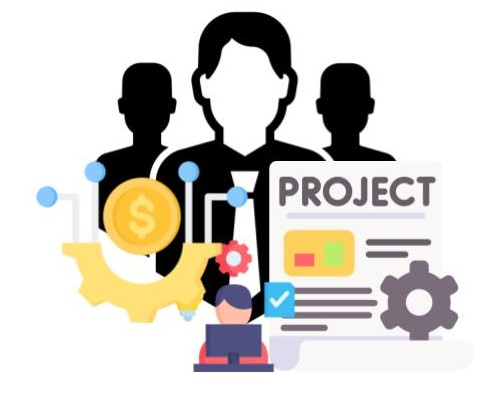
\includegraphics[width=0.6\textwidth]{figures/memoryCover.jpg}
\vspace*{1cm}

{\large Realizado por}\\
\textbf{\Large \tfgAuthors}

\vspace*{0.25cm}

\textbf{Para la asignatura}\\
{\large \tfgSubject}\\

\vspace*{0.2in}

\textbf{Dentro del}\\
{\large \tfgDegree}\\

\end{center}

\clearpage\setcounter{page}{1} % Comienza a incluir números de página a partir de aquí
\pagenumbering{roman} % En números romanos
    \chapter*{Resumen}

Resumen del portfolio

\vspace{.5cm}

\textbf{Palabras clave:} palabraClave1, palabraClave2, palabraClave3 ... 

    
    % Índice del documento y de figuras
    \begingroup
        % Los enlaces son normalmente azules, pero en los índices se configuran a negro para que no aparezca todo azul
        \hypersetup{linkcolor=black}
        \tableofcontents
        \listoffigures
        \listoftables
    \endgroup
    
    % Cambia el estilo de números de página de romanos a normal
    \clearpage\pagenumbering{arabic}
    
    % Capítulos del trabajo
    \chapter{Introducción}\label{cap:introduccion}

Introducción al portfolio
    \chapter{Presentación personal}\label{cap:presentacion-personal}

Experiencia previa y expectativas
    \chapter{Sesión X}\label{cap:sesionX}

\section{Conceptos y contenidos aprendidos}
Ahora conozco, comprendo, soy capaz de aplicar ...

\section{Preguntas realizadas al profesor}
Preguntas realizadas durante y/o después de la charla.

\section{Reflexión y progreso}
Sería capaz de aplicarlo en <escenario> -- Me ha merecido poco/mucho/... la pena porque ...

\section{De qué manera ayuda a la solución del caso de estudio}


    \chapter{Autoevaluación}\label{cap:autoevaluacion}

\section{Autoevaluación final}

\subsection{Conceptos y contenidos aprendidos}
Síntesis de los obtenidos en cada sesión.

\subsection{Competencias desarrolladas}
Ahora me siento competente para ... --- Para desarrollar la competencia ... hubiera necesitado ...

    \chapter{Reflexiones finales}\label{cap:reflexiones-finales}

\subsection{Conclusiones o Reflexiones iniciales}

\subsection{Justificación de la valoración del portfolio de los compañeros}

\subsection{Conclusiones adicionales tras la valoración del portfolio}
    \chapter{Autodeclaración uso de IA Generativa}\label{cap:uso-de-ia}

Exponer aquí el uso de IA

% Fin del documento
\end{document}
